\documentclass[conference]{IEEEtran}
\IEEEoverridecommandlockouts
\usepackage{cite}
\usepackage{amsmath,amssymb}
\usepackage{graphicx}
\usepackage{booktabs}
\usepackage{xcolor}
\usepackage{pgfplots}
\pgfplotsset{compat=1.16}
\usepackage[hidelinks]{hyperref}
\usepackage{url}

\begin{document}

\title{Early Warning of Product Quality Problems from Customer Reviews:\\
Which Products Should a Quality Team Investigate First?}

\author{\IEEEauthorblockN{Parth Arya, Vijay Krishna, Gautam Dadhich}
\IEEEauthorblockA{Big Data Analytics, Goa Institute of Management, Goa, India\\
B2026027, B2026053, B2026015}}

\maketitle

\begin{abstract}
A quality manager choosing 50 products to investigate faces two uncertainties. Will complaints increase, and will enough reviews arrive to establish whether they did? Using 2.03 million Amazon Appliances reviews, we evaluated both questions chronologically. In an archived benchmark on product-months with observable outcomes, validation-selected gradient boosting achieved test average precision of 0.304 versus 0.204 for a cumulative-sum control chart (CUSUM); that benchmark included a snapshot helpful-vote feature that would not have been available on the decision date. We then rebuilt each monthly queue using only information available when investigations would begin. Across 21 months and 1,050 slots, risk-only boosting identified 143 subsequent spikes in one- and two-star reviews and CUSUM identified 76. Multiplying predicted risk by the estimated probability of sufficient review coverage raised the count to 264, mainly by selecting products whose outcomes could be observed: precision among observable alerts fell from 42.4\% to 33.5\%. Because each outcome is defined within the month after the alert, confirmation necessarily falls inside that month; for confirmed hits the median was 17 days. The queue analysis was designed after the original test results were seen and should be read as exploratory. Establishing physical defects or avoided reputational damage requires independent evidence.
\end{abstract}

\begin{IEEEkeywords}
product quality, online reviews, early warning, alert prioritization, statistical process control
\end{IEEEkeywords}

\section{Introduction}
On 1 January a quality analyst might investigate a washing-machine listing with several reports of leaks, an appliance with a history of intermittent failures, or a new product with few reviews. Each choice uses an investigation slot. For some choices the following month brings too little feedback even to judge whether a warning was warranted. A deployment evaluation needs to count those slots.

We ask three questions. Can review history anticipate a rise in low ratings, and does text improve the forecast? Which ranking finds the most verifiable spikes for a fixed workload? On confirmed alerts, how soon within the month does the review evidence become conclusive? A quality analyst can use the resulting shortlist to inspect recurring complaints and cross-check returns, service tickets, installation problems or supplier records.

\section{Related Work and Project Contribution}
A retrospective search can begin with a complaint and ask which other customers describe the same failure. A quality analyst preparing next month's investigation list faces an earlier decision. The analyst has to choose a product before knowing whether customers will post enough reviews to reveal a change. This distinction affects which products enter the evaluation and what constitutes success.

Prior work identified defect-related signals in reviews and discussion threads \cite{abbas,abrahams,winkler}. Our unit is a product at the start of a month and the outcome comes from subsequent reviews. CUSUM accumulates deviations from a historical reference \cite{page}, making it a useful comparator for a team already tracking complaint trends. Recent volume provides another: it tests how far the team can get by investigating popular products alone. Our contribution is to evaluate each decision before outcomes are available, account for every slot, and record from dated reviews when each confirmed spike became observable.

\section{Data and Target}
The Appliances category of Amazon Reviews'23 \cite{hou,amazon} contained 2,128,605 raw reviews. Date filtering to January 2014--September 2023 removed 73,341 records. Deduplication on reviewer, parent product, timestamp, rating and body removed 21,840. The clean sample contains 2,033,424 reviews of 91,642 products. Variants share a parent product ID when available.

A product is eligible on the first day of a month if the two preceding full months contain five or more reviews. For a January decision, November and December form the principal feature window. Trends may also draw on the preceding two months and earlier product history. Let $b$ denote the past share of one- and two-star reviews, $n$ the target-month review count and $s$ the target-month low-rating share. The outcome is observable when $O=\mathbb{1}[n\ge 5]$. Among observable cases the event is
\begin{equation}
Y=\mathbb{1}\left[s\ge 0.30 \text{ and } s-b\ge 0.10\right].
\end{equation}
One low rating in ten past reviews followed by three in eight new reviews qualifies: the share rose from 10\% to 37.5\%. Three low ratings in four new reviews leave the outcome unresolved. A delivery delay, an inaccurate listing and a physical defect can all produce a spike.

Across the study, 174,868 product-months met the past-volume requirement and 72,977 had observable outcomes. In the test period 39,938 were eligible and 14,765 were observable (37.0\%). Table~\ref{tab:cohort} shows the rising event rate. Average precision must be interpreted alongside the prevalence in its evaluation period.

\begin{table}[t]
\caption{Observable Cohort by Decision Date. Products Can Appear in Several Months.}
\label{tab:cohort}
\centering\footnotesize
\begin{tabular}{@{}lrrr@{}}
\toprule
Period & Labelled & Events & Rate \\
\midrule
Train, 2014--2020 & 46,117 & 3,857 & 8.4\% \\
Validation, 2021 & 12,095 & 1,570 & 13.0\% \\
Test, 2022--Sep.\ 2023 & 14,765 & 2,317 & 15.7\% \\
\bottomrule
\end{tabular}
\end{table}

\begin{table}[t]
\caption{Archived Benchmark on Observable Cases. P@50 Is Precision After Restricting Candidates to Labelled Cases. These Models Include a Snapshot Helpful-Vote Feature Not Available at the Decision Date; the Queue Models in Tables~\ref{tab:replay}--\ref{tab:ledger} Exclude It.}
\label{tab:bench}
\centering\footnotesize
\begin{tabular}{@{}lccc@{}}
\toprule
Method & Val.\ AP & Test AP & P@50 \\
\midrule
High low-rating share & 0.165 & 0.185 & 0.171 \\
Rising low-rating share & 0.114 & 0.134 & 0.128 \\
CUSUM & 0.170 & 0.204 & 0.258 \\
Logistic, S & 0.255 & 0.279 & 0.359 \\
Logistic, S+A & 0.256 & 0.281 & 0.358 \\
Logistic, S+A+T & 0.260 & 0.287 & 0.365 \\
Boosting, S & 0.272 & 0.303 & 0.378 \\
Boosting, S+A & 0.276 & 0.304 & 0.385 \\
Boosting, S+A+T & 0.268 & 0.308 & 0.400 \\
\bottomrule
\end{tabular}
\end{table}

\section{Methods}
\subsection{Historical ranking benchmark}
We compared logistic regression and histogram gradient boosting \cite{friedman} with the past low-rating share, its change, and an upper CUSUM. Structured features (S) include volume, rating level and dispersion, changes from the preceding window, product age, and four CUSUM scores. The chart accumulates each month's low-rating share above the product's historical pooled rate, with a slack allowance and a floor of zero. Aspect features (A) summarize eight complaint categories including leaks, poor fit, damage and failure in use. The 27 features describe prevalence, change and prevalence among low-rated reviews. A positive mention of an easy refund can trigger the same keyword as a complaint, limiting interpretation.

Text features (T) use training-fitted TF--IDF unigrams and bigrams. Within each past month the implementation retains up to 25 reviews, lowest-rated first and then most recent, truncating each to 400 characters. Logistic regression uses sparse text features directly. Boosting uses 100 SVD components. Average precision (AP) summarizes precision and recall across thresholds in this rare-event task \cite{saito}. Historical models included the snapshot's aggregate helpful-vote count. Its value at the historical decision date cannot be reconstructed, so the archived benchmark in Table~\ref{tab:bench} may overstate what was achievable on the decision date. Permutation importance on the validation year suggests the effect is small: shuffling this feature reduced the selected model's average precision by about 0.003, and it ranked 13th of 43 inputs. We removed the feature from all newly fitted queue models.

\subsection{Decision-date replay}
In each test month, rank every product meeting the past-volume requirement. Select the highest $K$ scores, breaking ties by product ID, then join next-month outcomes. Each product can appear again in a later month. We use $K=50$ as the main scenario and 10, 100 and 200 as capacity checks.

The risk estimator $r(x)=P(Y=1\mid O=1,x)$ uses the structured-plus-aspect family selected in the original validation study. We fit observable training outcomes with 300 boosting iterations, learning rate 0.05 and L2 penalty 1. Validation AP selected 15 leaves from 15 and 31. The coverage estimator uses the same architecture and learns $P(O=1\mid x)$ from all eligible training windows. Its target is whether at least five subsequent reviews arrived. The additional ranking score estimates
\begin{equation}
q(x)=P(O=1\mid x)\,P(Y=1\mid O=1,x).
\end{equation}
This joint probability targets a verifiable spike. A product with high conditional risk but sparse feedback can move down the list. Comparators are CUSUM (validation-selected slack 0.05), recent review volume, and ascending prior low-rating share. The last rule tests whether arithmetic headroom for an increase explains performance on its own.

For $H$ confirmed spikes, $F$ observable non-events and $U$ unknown outcomes, confirmed yield is $H/(H+F+U)$. Precision among observable alerts is $H/(H+F)$. The first measures evidence obtained per investigation. An unresolved alert earns no credit toward verified yield and its underlying product condition remains unknown.

\subsection{How coverage changes the ranking}
Consider two hypothetical products. For the first, the estimated chance of sufficient follow-up is 0.20 and the conditional chance of a spike is 0.60. For the second, the estimates are 0.80 and 0.30. The first product ranks higher on conditional risk. The second ranks higher on expected verifiable yield, with a joint score of 0.24 versus 0.12. This multiplication follows the conditional probability rule and requires no independence assumption. A team with reliable warranty records for sparsely reviewed products might reasonably rank them differently because it has another means of verification.

The replay evaluates the ordering induced by these scores. It does not establish whether a score of 0.24 corresponds to a 24\% event frequency in a new deployment. A fixed monthly capacity only requires an ordering. Using the scores to estimate staffing needs or to trigger action at a fixed probability would also require checking calibration over time.

\section{Results}
\subsection{Review history and the contribution of text}
Validation-selected boosting (S+A) reached 0.304 test AP (95\% month-bootstrap interval 0.283--0.327), against 0.204 for CUSUM and 0.157 test prevalence. These archived figures include the snapshot helpful-vote feature, so they may slightly overstate decision-date performance (Section~IV-A); the queue results below do not use it. Full-text boosting reached 0.308 on test but scored lower on validation (Table~\ref{tab:bench}). Adding aspects and text to structured inputs gained 0.005 AP for boosting, with a paired interval of $-0.005$ to $+0.018$, and 0.008 for logistic regression. Complaint themes can direct investigators to relevant reviews; the evidence for a ranking gain from text is limited.

The rising-share rule produced ROC-AUC 0.423. Regression toward typical complaint rates offers one explanation. The target also requires a further rise from the current baseline, making another qualifying increase mechanically harder after an unusually bad recent window.

\begin{figure}[t]
\centering
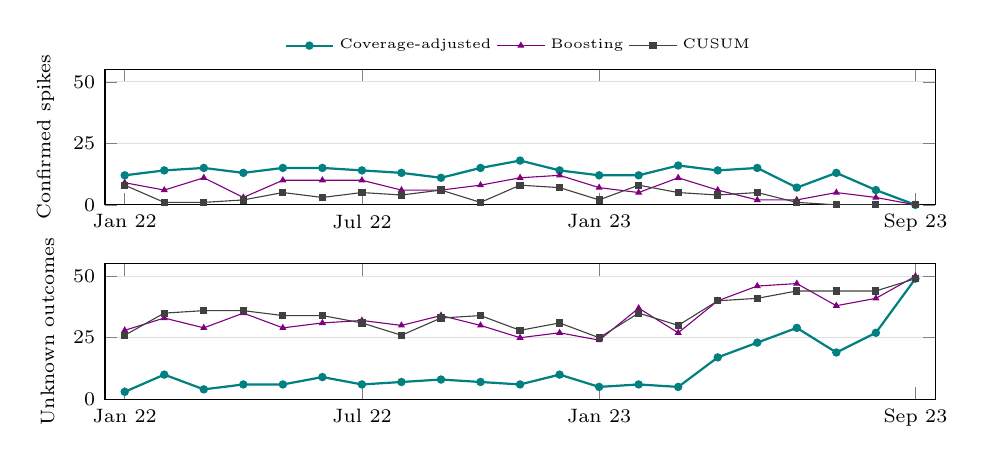
\begin{tikzpicture}
\pgfplotsset{
  queue/.style={width=\columnwidth, height=3.3cm, xmin=0.5, xmax=21.5,
    ymin=0, ymax=55, ytick={0,25,50},
    xtick={1,7,13,21}, xticklabels={Jan 22,Jul 22,Jan 23,Sep 23},
    tick label style={font=\scriptsize}, label style={font=\scriptsize},
    ymajorgrids, grid style={black!12}, mark size=1.1pt}}
\begin{axis}[queue, name=top, ylabel={Confirmed spikes},
    legend style={font=\tiny, at={(0.5,1.04)}, anchor=south, legend columns=3, draw=none},
    legend cell align=left]
\addplot[teal, thick, mark=*] coordinates {(1,12)(2,14)(3,15)(4,13)(5,15)(6,15)(7,14)(8,13)(9,11)(10,15)(11,18)(12,14)(13,12)(14,12)(15,16)(16,14)(17,15)(18,7)(19,13)(20,6)(21,0)};
\addplot[violet, mark=triangle*] coordinates {(1,9)(2,6)(3,11)(4,3)(5,10)(6,10)(7,10)(8,6)(9,6)(10,8)(11,11)(12,12)(13,7)(14,5)(15,11)(16,6)(17,2)(18,2)(19,5)(20,3)(21,0)};
\addplot[black!75, mark=square*] coordinates {(1,8)(2,1)(3,1)(4,2)(5,5)(6,3)(7,5)(8,4)(9,6)(10,1)(11,8)(12,7)(13,2)(14,8)(15,5)(16,4)(17,5)(18,1)(19,0)(20,0)(21,0)};
\legend{Coverage-adjusted, Boosting, CUSUM}
\end{axis}
\begin{axis}[queue, at={(top.south)}, anchor=north, yshift=-0.75cm, ylabel={Unknown outcomes}]
\addplot[teal, thick, mark=*] coordinates {(1,3)(2,10)(3,4)(4,6)(5,6)(6,9)(7,6)(8,7)(9,8)(10,7)(11,6)(12,10)(13,5)(14,6)(15,5)(16,17)(17,23)(18,29)(19,19)(20,27)(21,49)};
\addplot[violet, mark=triangle*] coordinates {(1,28)(2,33)(3,29)(4,35)(5,29)(6,31)(7,32)(8,30)(9,34)(10,30)(11,25)(12,27)(13,24)(14,37)(15,27)(16,40)(17,46)(18,47)(19,38)(20,41)(21,50)};
\addplot[black!75, mark=square*] coordinates {(1,26)(2,35)(3,36)(4,36)(5,34)(6,34)(7,31)(8,26)(9,33)(10,34)(11,28)(12,31)(13,25)(14,35)(15,30)(16,40)(17,41)(18,44)(19,44)(20,44)(21,49)};
\end{axis}
\end{tikzpicture}
\caption{Monthly outcomes of the 50-slot queue. Sparse follow-up near the end of the test period increases the number of unresolved alerts.}
\label{fig:monthly}
\end{figure}

\subsection{What 50 investigations actually return}
Table~\ref{tab:replay} uses every product eligible at decision time. Risk-only boosting recorded 143 hits and 713 unknowns. Among its observable alerts, precision was 42.4\%. Across all issued slots, confirmed yield was 13.6\%. Choosing on volume alone produced 101 hits. Ranking by low prior share alone found 18.

Coverage-adjusted ranking produced 264 hits, 524 observable non-events and 262 unknowns. Its precision among observable alerts was 33.5\%. A larger share of its queue could be evaluated, raising confirmed yield to 25.1\%. The gain over risk-only ranking therefore came from fewer unresolved alerts (262 against 713), not from higher precision: among alerts that could be evaluated, risk-only ranking was more often right. Volume alone, which also favours products likely to receive feedback, found 101 hits at 10.5\% observable precision, so coverage accounts for part of the gain but not all of it. Compared with CUSUM, coverage-adjusted ranking provided 9.0 additional confirmed spikes per month and had more hits in 20 of 21 months. A paired circular block bootstrap (three consecutive months per block, 5,000 draws, seed 42) gave an indicative 95\% interval of 7.3 to 10.4 additional hits per month. This interval describes variation within the replay, conditional on the fitted models. Fig.~\ref{fig:tradeoff} places each policy by verified yield and observable precision.

\begin{figure}[t]
\centering
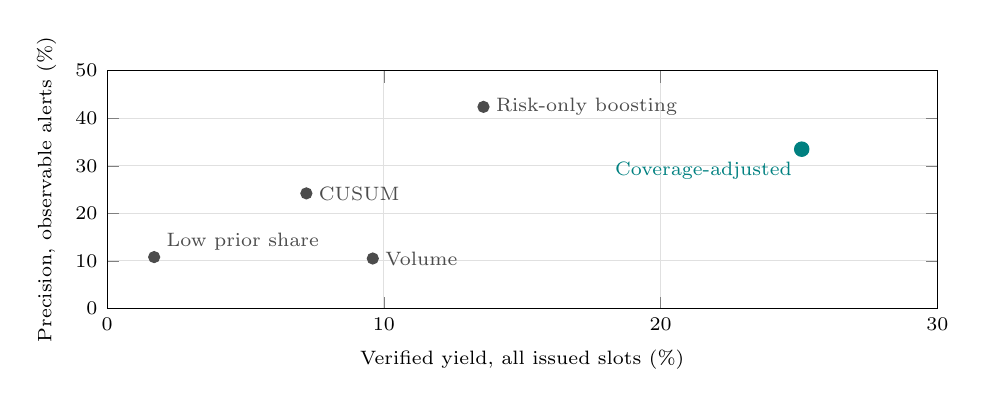
\begin{tikzpicture}
\begin{axis}[width=\columnwidth, height=4.6cm,
    xmin=0, xmax=30, ymin=0, ymax=50,
    xtick={0,10,20,30}, ytick={0,10,20,30,40,50},
    xlabel={Verified yield, all issued slots (\%)},
    ylabel={Precision, observable alerts (\%)},
    tick label style={font=\scriptsize}, label style={font=\scriptsize},
    grid=major, grid style={black!12},
    nodes near coords, point meta=explicit symbolic,
    every node near coord/.append style={font=\scriptsize, anchor=west, xshift=1pt}]
\addplot[only marks, mark=*, mark size=2pt, black!70] coordinates {
    (7.2,24.2) [CUSUM]
    (9.6,10.5) [Volume]
    (13.6,42.4) [Risk-only boosting]
};
\addplot[only marks, mark=*, mark size=2pt, black!70,
    every node near coord/.append style={anchor=south west, yshift=-1pt}] coordinates {
    (1.7,10.8) [Low prior share]
};
\addplot[only marks, mark=*, mark size=2.6pt, teal,
    every node near coord/.append style={anchor=north east, xshift=-1pt, yshift=-1pt}] coordinates {
    (25.1,33.5) [Coverage-adjusted]
};
\end{axis}
\end{tikzpicture}
\caption{Each policy's 50-slot queue over 21 months. Coverage-adjusted ranking confirms more spikes per issued slot, but a smaller share of its observable alerts are spikes than under risk-only boosting.}
\label{fig:tradeoff}
\end{figure}


At 200 slots, coverage-adjusted ranking finds 817 confirmed events, or 35.3\% of all 2,317 known test events. At 50 the corresponding share is 11.4\%. A manager can reach more events with additional investigations at diminishing yield per slot (Table~\ref{tab:capacity}). Fig.~\ref{fig:monthly} shows the month-to-month variation behind the averages.

\begin{table*}[t]
\caption{Decision-Date Replay over 21 Months. Unknown Denotes Fewer than Five Reviews in the Target Month. Verified Yield Uses All Issued Slots; Observable Precision Excludes Unknowns.}
\label{tab:replay}
\centering\footnotesize
\begin{tabular}{@{}lrrrrrr@{}}
\toprule
Policy & Issued & Confirmed spike & Observable non-event & Unknown & Verified yield (\%) & Observable precision (\%) \\
\midrule
CUSUM & 1,050 & 76 & 238 & 736 & 7.2 & 24.2 \\
Volume & 1,050 & 101 & 861 & 88 & 9.6 & 10.5 \\
Low prior share & 1,050 & 18 & 148 & 884 & 1.7 & 10.8 \\
Boosting & 1,050 & 143 & 194 & 713 & 13.6 & 42.4 \\
Coverage-adjusted & 1,050 & 264 & 524 & 262 & 25.1 & 33.5 \\
\bottomrule
\end{tabular}
\end{table*}

\subsection{Time to confirmation}
For each confirmed hit we reconstructed the cumulative count and low-rating share after each review day. We located the first day on which all criteria were met and remained satisfied through month-end. A January 1 alert first meeting and sustaining the criterion on January 18 is confirmed after 17 days. Among the 264 confirmed coverage-adjusted alerts the median was 17 days (interquartile range 12--24). Because the outcome window is the month that begins on the decision date, this interval cannot exceed about 30 days by construction. It describes how quickly confirming reviews arrived, not how far ahead of a developing problem the alert came. Defect onset and time required for investigators to act remain unknown. Fig.~\ref{fig:confirm} shows the full distribution; about one in eight confirmations came within the first week and about one in five after day 24.

\begin{figure}[t]
\centering
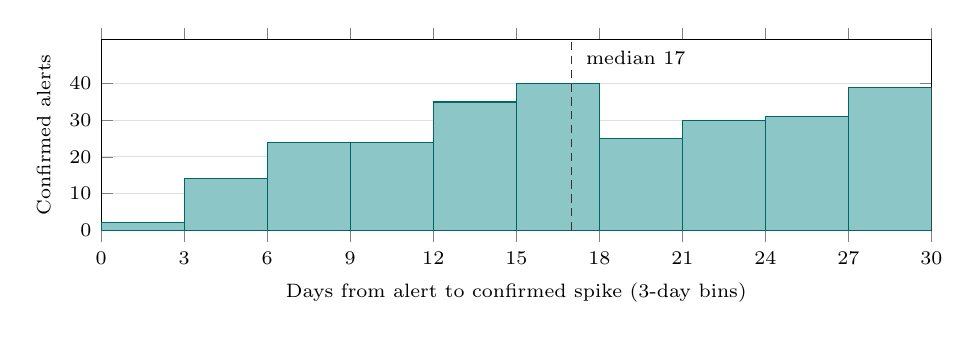
\begin{tikzpicture}
\begin{axis}[width=\columnwidth, height=4.0cm,
    ybar, bar width=3, bar shift=0, xmin=0, xmax=30, ymin=0, ymax=52,
    xtick={0,3,...,30}, ytick={0,10,20,30,40},
    xticklabel style={font=\scriptsize}, yticklabel style={font=\scriptsize},
    xlabel={Days from alert to confirmed spike (3-day bins)},
    ylabel={Confirmed alerts},
    label style={font=\scriptsize},
    ymajorgrids, grid style={black!12}]
\addplot[fill=teal!45, draw=teal!80!black] coordinates {
    (1.5,2) (4.5,14) (7.5,24) (10.5,24) (13.5,35) (16.5,40) (19.5,25) (22.5,30) (25.5,31) (28.5,39)};
\end{axis}
\begin{axis}[width=\columnwidth, height=4.0cm, xmin=0, xmax=30, ymin=0, ymax=52,
    axis lines=none, ticks=none]
\draw[densely dashed, black!80] (axis cs:17,0) -- (axis cs:17,52);
\node[font=\scriptsize, anchor=west, inner sep=1pt, fill=white] at (axis cs:17.4,47) {median 17};
\end{axis}
\end{tikzpicture}
\caption{Time to confirmation for the 264 confirmed coverage-adjusted alerts. The last bin includes day 30. Because the outcome window is the month beginning on the decision date, no value can exceed about 30 days.}
\label{fig:confirm}
\end{figure}


\begin{table}[t]
\caption{Confirmed Spikes per 100 Issued Slots by Monthly Capacity.}
\label{tab:capacity}
\centering\footnotesize
\begin{tabular}{@{}rccc@{}}
\toprule
$K$ & CUSUM & Risk-only & Coverage-adjusted \\
\midrule
10 & 7.6 & 14.8 & 28.6 \\
50 & 7.2 & 13.6 & 25.1 \\
100 & 7.2 & 13.3 & 23.1 \\
200 & 7.1 & 12.3 & 19.5 \\
\bottomrule
\end{tabular}
\end{table}

\begin{table}[t]
\caption{Selected Entries from the 1 January 2022 Alert Ledger. The Score Is the Estimated Joint Probability Used for Ranking.}
\label{tab:ledger}
\centering\footnotesize
\begin{tabular}{@{}rlcl@{}}
\toprule
Rank & Product ID & Score & Outcome \\
\midrule
1 & B0C4TLWPCD & 0.393 & Observable non-event \\
3 & B0B9CCJTDF & 0.354 & Confirmed spike \\
7 & B00OO9U8QY & 0.322 & Unknown \\
\bottomrule
\end{tabular}
\end{table}

\subsection{Tracing three alerts from one decision date}
On 1 January 2022, the first, third and seventh products in the coverage-adjusted queue illustrate the three possible outcomes (Table~\ref{tab:ledger}). The highest-ranked product accumulated enough reviews to evaluate, but its final low-rating share did not satisfy both spike criteria. The third-ranked product met the sustained threshold on 10 January, nine days after selection. The seventh-ranked product had too few reviews to evaluate by month-end. Each selection consumed one of the same 50 slots. Treating the seventh as a confirmed negative would imply evidence that the review record cannot supply.

\subsection{Which investigations does extra capacity buy?}
The capacity scenarios rank the same candidates with the same score. Subtracting the cumulative counts therefore measures what the next group of slots contributed. Across 21 months the first ten slots per month found 60 spikes in 210 investigations. Ranks 11--50 added 204 in 840, ranks 51--100 added 222 in 1,050, and ranks 101--200 added 331 in 2,100. The last group still found cases, but required about 6.3 investigations per additional verified spike. The first ten slots required 3.5. This difference matters when the manager has discretion over the last analyst shift of the month.

The 1,050 coverage-adjusted alerts corresponded to 388 distinct products. The 264 confirmed product-months involved 170 distinct products. Repeated alerts could represent persistent complaints, recurrence after an earlier improvement, or overlapping evidence across consecutive decisions. The ledger cannot distinguish these explanations. A team that opens a single case per product would face a different workload. Its policy would need a rule for reopening an existing case before the replay could estimate staffing requirements.

\subsection{When the queue became harder to verify}
In the twelve test months of 2022, 169 of the 600 coverage-adjusted alerts became confirmed spikes and 82 remained unknown. In the nine test months of 2023, 95 of 450 became confirmed spikes and 180 remained unknown. Verified yield fell from 28.2\% to 21.1\%, while the unresolved share rose from 13.7\% to 40.0\%. Among alerts with sufficient feedback, the corresponding spike shares were 32.6\% and 35.2\%. A manager looking only at observable alerts would miss the deterioration in yield per issued slot. The periods cover different calendar months, and the archive ends in September. These data alone cannot establish the cause of the change.

\section{Business Interpretation and Limitations}
A team seeking verifiable signals per investigation obtained about one confirmed spike per four slots under coverage-adjusted ranking. Optimizing for review coverage favors products receiving regular feedback, and it lowered precision among observable alerts, so the gain reflects how measurable a product's outcome is as much as how risky the product is. A team responsible for low-volume or emerging products could reserve slots for them and use returns or support tickets to verify outcomes. Repeated complaints about an incompatible part might prompt a listing correction, while repeated reports of a unit failing in use might warrant a batch check.

Products recur and adjacent feature windows overlap. Month-block resampling preserves some dependence, but the study covers one category and includes sparse late months. We designed the queue extension after inspecting the original benchmark on these dates, and we did not repeat the replay on the 2021 validation year before scoring the test months. The choice of the coverage-adjusted score was therefore not validated in advance, and the queue results should be read as an exploratory, retrospective comparison. Performance on later dates, unfamiliar products and other categories remains open. The original sensitivity grid yielded positive rates from 8.9\% to 15.9\% as minimum volumes and required increases changed. Those counts establish how often the target occurs. Each alternative definition would require a separate queue evaluation to establish the policy ranking.

Financial savings, independently confirmed defects and reputational changes were outside the available data. A prospective pilot could log analyst minutes, evidence, issue type, action date and disposition for each alert, alongside a sample outside the queue. Cost per independently confirmed issue would provide a direct test of business value.

\subsection{A prospective test for the quality team}
Before each monthly review, the team could save the full eligible list, the scores available on that date and its staffing limit. For each investigation the analyst would record the suspected issue, minutes spent, supporting evidence and decision date. A repeated alert for an open case would be linked to the original investigation. Closing a case would require a recorded disposition, such as a verified listing error, a service issue, a confirmed product defect or insufficient evidence. These categories would let the team compare the review-based signal with the issue that actually required action.

For a comparison with current practice, the team could investigate products selected by both policies once and sample from the products on which the policies disagree. Recording the sampling probabilities would allow separate estimates for the two queues. Where feasible, investigators could review the evidence without seeing which method selected the product. The primary business measure would be independently confirmed issues per analyst-hour. Time from selection to corrective action and the share of unresolved investigations would help explain changes in that measure. These are proposed pilot outcomes. The historical review archive contains neither analyst time nor corrective actions.

\section{Reproducibility}
The team repository \cite{repo} contains the original analysis and benchmark outputs (base revision 571955b). The accompanying revision includes decision-date feature construction, the alert ledger, dated threshold crossings and table generation. The historical benchmark is reported from archived outputs. The new queue models were fitted from the official raw review archive. The reconstructed clean-review and labelled-window counts matched the original report. Commands and pinned dependencies are supplied with the code.

\subsection{Checks against the released outputs}
The accompanying code update adds \texttt{src/08\_decision\_queue.py} and \texttt{src/09\_warning\_time.py}. From the repository root, use the commands below after installing the project requirements. The first three commands prepare the review windows and their decision-date features. The last two generate the queue ledger and the dates used for the time-to-confirmation calculation.

{\footnotesize
\begin{verbatim}
python src/01_download.py
python src/02_build_windows.py
python src/04_features.py --decision-queue
python src/08_decision_queue.py
python src/09_warning_time.py
\end{verbatim}}

Three checks connect these outputs to the results. First, each policy at capacity 50 should have 50 distinct product IDs on each of 21 decision dates. Second, grouping its ledger by outcome should reproduce Table~\ref{tab:replay}, including the unknown category. Third, joining the confirmed coverage-adjusted alerts to the crossing dates by product, decision date and policy should return 264 rows. Subtracting each decision date from its crossing date should give the reported median of 17 days. These checks separate differences in candidate selection from differences in outcome counting.

\subsection{AI Use Declaration}
AI tools (Anthropic's Claude and OpenAI's Codex) were used throughout this project. They wrote most of the data-processing, modelling and evaluation code; designed, implemented and ran the decision-date replay and the time-to-confirmation analysis; generated the tables and figure; and drafted much of the report text, including the revisions in this version. The authors ran and checked the code, verified every reported number against the generated output files, checked every reference, and take responsibility for the submission.

\section{Conclusion}
Accounting for the probability of sufficient review coverage raised verifiable spikes from 143 to 264 at the same 1,050-slot budget, chiefly by choosing products whose outcomes could be observed; precision among observable alerts fell from 42.4\% to 33.5\%. Confirmed spikes became observable a median of 17 days after selection, a figure bounded by the one-month outcome window. Because the queue design followed inspection of the test period, a prospective study is needed to establish whether this ranking helps investigators confirm and resolve customer issues.

{\footnotesize
\begin{thebibliography}{00}
\bibitem{abbas} Y. Abbas and M. S. I. Malik, ``Defective products identification framework using online reviews,'' \emph{Electronic Commerce Research}, vol. 23, no. 2, pp. 899--920, 2023, doi: 10.1007/s10660-021-09495-8.
\bibitem{abrahams} A. S. Abrahams, W. Fan, G. A. Wang, Z. Zhang, and J. Jiao, ``An integrated text analytic framework for product defect discovery,'' \emph{Production and Operations Management}, vol. 24, no. 6, pp. 975--990, 2015, doi: 10.1111/poms.12303.
\bibitem{winkler} M. Winkler, A. S. Abrahams, R. Gruss, and J. P. Ehsani, ``Toy safety surveillance from online reviews,'' \emph{Decision Support Systems}, vol. 90, pp. 23--32, 2016, doi: 10.1016/j.dss.2016.06.016.
\bibitem{page} E. S. Page, ``Continuous inspection schemes,'' \emph{Biometrika}, vol. 41, no. 1/2, pp. 100--115, 1954.
\bibitem{hou} Y. Hou, J. Li, Z. He, A. Yan, X. Chen, and J. McAuley, ``Bridging language and items for retrieval and recommendation,'' arXiv preprint arXiv:2403.03952 [cs.IR], Mar. 2024. [Online]. Available: https://arxiv.org/abs/2403.03952
\bibitem{amazon} McAuley Lab, ``Amazon Reviews'23: Dataset documentation,'' 2024. [Online]. Available: https://amazon-reviews-2023.github.io/
\bibitem{friedman} J. H. Friedman, ``Greedy function approximation: A gradient boosting machine,'' \emph{Annals of Statistics}, vol. 29, no. 5, pp. 1189--1232, 2001.
\bibitem{saito} T. Saito and M. Rehmsmeier, ``The precision-recall plot is more informative than the ROC plot when evaluating binary classifiers on imbalanced datasets,'' \emph{PLoS ONE}, vol. 10, no. 3, Art. no. e0118432, 2015, doi: 10.1371/journal.pone.0118432.
\bibitem{repo} P. Arya, V. Krishna, and G. Dadhich, ``Quality warning: Analysis code and archived results,'' GitHub repository, 2026. [Online]. Available: https://github.com/Gautam-dadhich/quality-warning
\end{thebibliography}}

\end{document}
